\documentclass[12pt]{article}
\usepackage{graphicx}
\usepackage{caption}
\usepackage{subcaption}
\usepackage{float}
\usepackage{fancyhdr}
\usepackage{epstopdf}				
\usepackage{multicol}
\usepackage{chngcntr}
\usepackage{amsmath}
\usepackage{mathtools}
\usepackage{caption}
\usepackage{subcaption}
\usepackage[letterpaper, headsep=0.5in]{geometry}
\usepackage[colorlinks=true, allcolors=black]{hyperref}

\usepackage{listings}
\usepackage{mcode}
\providecommand{\MATLAB}[1]{\lstinputlisting{#1}}

\usepackage [autostyle, english = american]{csquotes}
\MakeOuterQuote{"}

%%%%%%%%%%%%%%%%%%%%%%%%%%%%%%%%%%%%%%%%%%%%%%%%%%%%%%%%%%%%%%%%%%%%%%%%%%%%%%%%%%%%%%%%%%%%%%%%%%%%%%%%%%%%%%%%%%%%%%%%%%%%
%%%%%%%%%%%%%%%%%%%%%%%%%%%%%%%%%%%%%%%%%%%%%%%%  Custom Commands   %%%%%%%%%%%%%%%%%%%%%%%%%%%%%%%%%%%%%%%%%%%%%%%%%%%%%%%%
%%%%%%%%%%%%%%%%%%%%%%%%%%%%%%%%%%%%%%%%%%%%%%%%%%%%%%%%%%%%%%%%%%%%%%%%%%%%%%%%%%%%%%%%%%%%%%%%%%%%%%%%%%%%%%%%%%%%%%%%%%%%

% New definition of square root:
% it renames \sqrt as \oldsqrt
\let\oldsqrt\sqrt
% it defines the new \sqrt in terms of the old one
\def\sqrt{\mathpalette\DHLhksqrt}
\def\DHLhksqrt#1#2{%
\setbox0=\hbox{$#1\oldsqrt{#2\,}$}\dimen0=\ht0
\advance\dimen0-0.2\ht0
\setbox2=\hbox{\vrule height\ht0 depth -\dimen0}%
{\box0\lower0.4pt\box2}}

\providecommand{\e}[1]{\ensuremath{\times 10^{#1}}}
\providecommand{\un}[1]{\ensuremath{\text{ #1}}}
\providecommand{\PerDiff}[3]{\begin{equation}\frac{2|#1 - #2|}{#1 + #2}\to #3\% \text{ diff.}\end{equation}}
\providecommand{\vect}[1]{\ensuremath{\utilde{#1}}}
\providecommand{\Problem}[2]{\setcounter{section}{#1}\section{#2-1}}

% Keep floats in sections
\usepackage{placeins}

\let\Oldsection\section
\renewcommand{\section}{\FloatBarrier\Oldsection}

\let\Oldsubsection\subsection
\renewcommand{\subsection}{\FloatBarrier\Oldsubsection}

\let\Oldsubsubsection\subsubsection
\renewcommand{\subsubsection}{\FloatBarrier\Oldsubsubsection}

% Set Header
\usepackage{fancyhdr}
\pagestyle{fancy}
\fancyhf{}
\rhead{
	NOT APPROVED\\
	Alexius Wadell: Rolling Eccentric Cylinder\\
	MAE 5730 Intermediate Dynamics and Vibrations
}


\begin{document}
\section{Problem Setup}
Consider a cylinder with radius of $R$, rolls without slip down a ramp with a slope of $\gamma$.
The center of mass of the cylinder has been offset from the center ($C$) by a distance $d < R$.
The total mass of the cylinder is $M$ and it has a moment of inertia $I^G$ about it's center of mass $G$.

\begin{figure}[h]
\centering
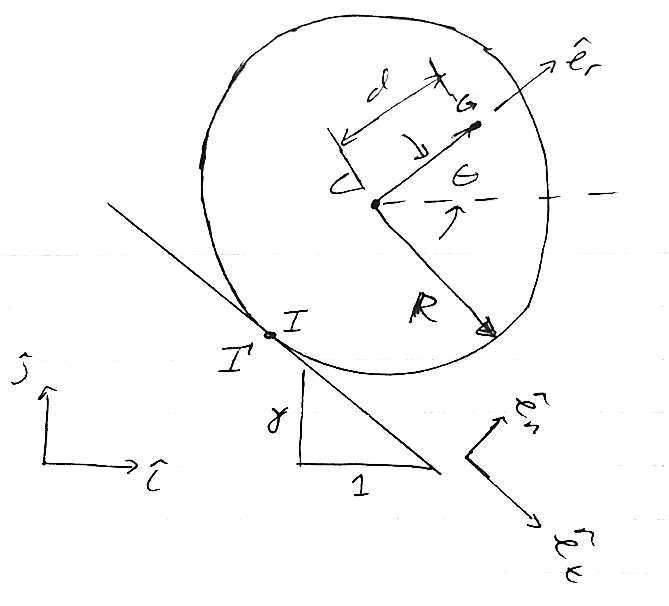
\includegraphics[height=2.5in]{img/problem_def.png}
\caption{Diagram of rolling eccentric cylinder problem}
\label{fig:problem_def}
\end{figure}

As shown in figure \ref{fig:problem_def}, there are three main reference frames for this problem.
The inertial frame defined by $\hat{i}$, $\hat{j}$ and $\hat{k}$.
The rotated inertial frame defined by $\hat{e}_n$ (normal to the ramp), $\hat{e}_t$ (tangent to the ramp) and $\hat{k}$.
\begin{equation}
\gamma_r = tan^{-1}(\gamma)
\end{equation}
\begin{equation}
\hat{e}_n =	\begin{bmatrix} sin(\gamma_r) \\ cos(\gamma_r) \\0 \end{bmatrix}
\end{equation}
\begin{equation}
\hat{e}_t =	\hat{e}_n \times \hat{k}
\end{equation}
And finally the rotating frame fixed to the center of the cylinder defined by $\hat{e}_r$ (Points to COM), $\hat{e}_\theta$ and $\hat{k}$.
\begin{equation}
\hat{e}_n =	\begin{bmatrix} cos(\theta) \\ sin(\theta) \\0 \end{bmatrix}
\end{equation}
\begin{equation}
\hat{e}_{\theta} =	\hat{k} \times \hat{e}_r
\end{equation}

We can now define the locations of the major points of interest for the problem in terms of these reference frames (Table \ref{tab:LocationDefs}).
\begin{table}[h]
\centering
\begin{tabular}{lc}
Item of Interest			& Definition \\\hline
Center of the Cylinder (C)	& $\vec{r}_{C/O} = x\hat{i} + y \hat{j}$\\
Contact Point (I)			& $\vec{r}_{I/C} = -R \hat{e}_n$\\
Center of Mass (G)			& $\vec{r}_{G/C} = -d \hat{e}_r$\\
G in Fixed Frame			& $\vec{r}_{G/O} = \vec{r}_{G/C} + \vec{r}_{C/O}$ \\
I relative to G				& $\vec{r}_{I/G} = \vec{r}_{I/C} - \vec{r}_{G/C}$ \\
\end{tabular}
\caption{Positions of items of interest for the problem}
\label{tab:LocationDefs}
\end{table}

Finally we can define the contact force acting at $I$ as $\vec{F} = F_n \hat{e}_n + F_t \hat{e}_t$.

\section{Equations of Motion}
We can now solve this system using Differential Algebraical Expression to solve for the 5 unknowns of the system: $\ddot{x}$, $\ddot{y}$, $\ddot{\theta}$, $F_n$ and $F_t$.
The angular momentum balance about $G$ (Eq. \ref{eq:AMB}) and the linear momentum balance for the cylinder (Eq. \ref{eq:LMB}), gives three of the five equations need for the DAE method.
\begin{equation}\label{eq:AMB}
\vec{r}_{I/G} \times \vec{F} = I^G\ddot{\theta} \hat{k}
\end{equation}
\begin{equation}\label{eq:LMB}
M \ddot{\vec{r}}_{G/O} = -Mg \cdot\hat{j} + \vec{F}
\end{equation}

The final two constraints on the systems is that cylinder shall not penetrate the ramp (Eq \ref{eq:noPenetration}) and the cylinder shall role without slip (Eq. \ref{eq:noSlip}), which once differentiated give the final two equations (Eq \ref{eq:noPenetration_dd} and \ref{eq:noSlip_dd}). 
\begin{equation}\label{eq:noPenetration}
\vec{r}_{C/O} \cdot \hat{e}_n = R
\end{equation}
\begin{equation}\label{eq:noSlip}
\dot{\vec{r}}_{C/O} \cdot \hat{e}_t = -R\dot{\theta}\hat{e}_t
\end{equation}

\begin{equation}\label{eq:noPenetration_dd}
\ddot{\vec{r}}_{C/O} \cdot \hat{e}_n =  0
\end{equation}
\begin{equation}\label{eq:noSlip_dd}
\ddot{\vec{r}}_{C/O} \cdot \hat{e}_t = -R\ddot{\theta}\hat{e}_t
\end{equation}

Using MATLAB to handle the differentiation and rearrangement of terms gives the following equation of motion for the system:
\begin{equation}\label{eq:eom_dae}
x = A^{-1}b
\end{equation}
\begin{equation}
A = \begin{bsmallmatrix}
	M & 0 & -M\,d\,\sin(\theta) & -\frac{\gamma}{\sqrt{{\gamma}^2+1}} & -\frac{1}{\sqrt{{\gamma}^2+1}}\\
	 0 & M & M\,d\,\cos(\theta) & -\frac{1}{\sqrt{{\gamma}^2+1}} & \frac{\gamma}{\sqrt{{\gamma}^2+1}}\\
	 0 & 0 & -I & -\frac{d\,\left(\cos(\theta)-\gamma\,\sin(\theta)\right)}{\sqrt{{\gamma}^2+1}} & \frac{\frac{R}{\sqrt{{\gamma}^2+1}}+d\,\sin(\theta)}{\sqrt{{\gamma}^2+1}}+\frac{\gamma\,\left(d\,\cos(\theta)+\frac{R\,\gamma}{\sqrt{{\gamma}^2+1}}\right)}{\sqrt{{\gamma}^2+1}}\\
	 1 & 0 & \frac{R}{\sqrt{{\gamma}^2+1}} & 0 & 0\\
	 0 & 1 & -\frac{R\,\gamma}{\sqrt{{\gamma}^2+1}} & 0 & 0 
\end{bsmallmatrix}
\end{equation}
\begin{equation}
x = \begin{bmatrix}
	\ddot{x}\\
	\ddot{y}\\
	\ddot{\theta}\\
	F_n \\
	F_t \\
\end{bmatrix}
\end{equation}

\begin{equation}
b = \begin{bmatrix}
\dot{\theta}^2\,M\,d\, \cos(\theta)\\
-M\,\left(g-\dot{\theta}^2\,d,\sin(\theta) \right)\\
0\\
0\\
0 \\
\end{bmatrix}
\end{equation}

\section{Numerical Simulation}
Using the derived equations of motion (Eq \ref{eq:eom_dae}), the cylinder was simulated using ode45 from rest, through the cylinder taking off.
Events were used to monitor the normal force ($F_n$), and the simulation was stopped once $F_n < 0$, as the ramp can not exert a negative normal force, thus indicating that the cylinder has taken off.

For the simulation and the rest of the present analysis the following parameters were used.
\begin{table}[h]
\centering
\begin{tabular}{cc}
Parameter	&	Value \\\hline
$I^G$		& 15 \\
$M$			& 20 \\
$R$			& 1  \\
$d$			& 0.4\\
$g$			& 10 \\
$\gamma$	& 1  \\
$\theta(0)$	& 0  \\\hline
\end{tabular}
\caption{Parameters used for Simulation}
\label{tab:SimParameters}
\end{table}

\section{Sanity Checks}
\subsection{Conservation of Energy}

The kinetic energy of the system is defined as:
\begin{equation}
E_k = \frac{I^G}{2}  \dot{\theta}^2 + \frac{M}{2} \left|\dot{\vec{r}}_{G/O} \right|^2
\end{equation}
\begin{equation}
E_k = 
\frac{I^G}{2}\dot{\theta}^2 +
\frac{M}{2} \left(
	\left( \dot{y} + d\dot{\theta} cos(\theta) \right)^2 +
	\left( \dot{x} - d\dot{\theta} sin(\theta) \right)^2
\right)
\end{equation}

The potential energy was defined based on the height of the center of mass ($G$), as this results in the shortest possible formula.
\begin{equation}
E_p = M g \cdot (\vec{r}_{G/O} \cdot \hat{j}) \to M g \cdot \left(y + d sin(\theta) \right)
\end{equation}

The kinetic energy ($E_k$), potential energy ($E_p$) and total energy ($E_p$) for the system was then computed for each time step returned by ode45 as shown in Figure \ref{fig:energy_con}.

Over the entire duration of the simulation the variation of the total energy ($E_t = E_k + E_p$), was 5.9\e{-9}.5.9\e{-9}
That is the max error deviation from perfect energy conservation was 5.9\e{-9}, indicating that the equations of motion respect energy conservation.
\begin{figure}[h]
\centering
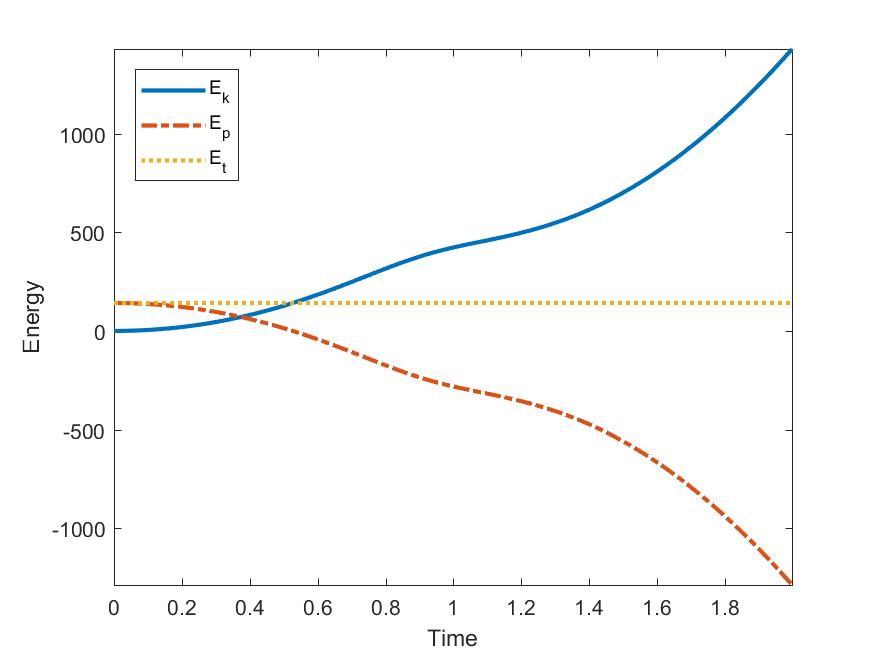
\includegraphics[height=3in]{img/energy_con.png}
\caption{System Energy showing Conservation of Total Energy to within 5.9\e{-9}}
\label{fig:energy_con}
\end{figure}

\subsection{Constraint Violations}
The velocity of the contact point ($I$) relative to the ramp, was also computed to verify that the no slip constraint was respected.
As shown in figure \ref{fig:constraint_check}, the contact point $I$ had a velocity relative to the slope of at most $8.8\e{-15}$, prior to lift of from the slope.
Again this gives a high degree of confidence, that the numerical solution satisfies the constraint equations.

\begin{figure}[h]
\centering
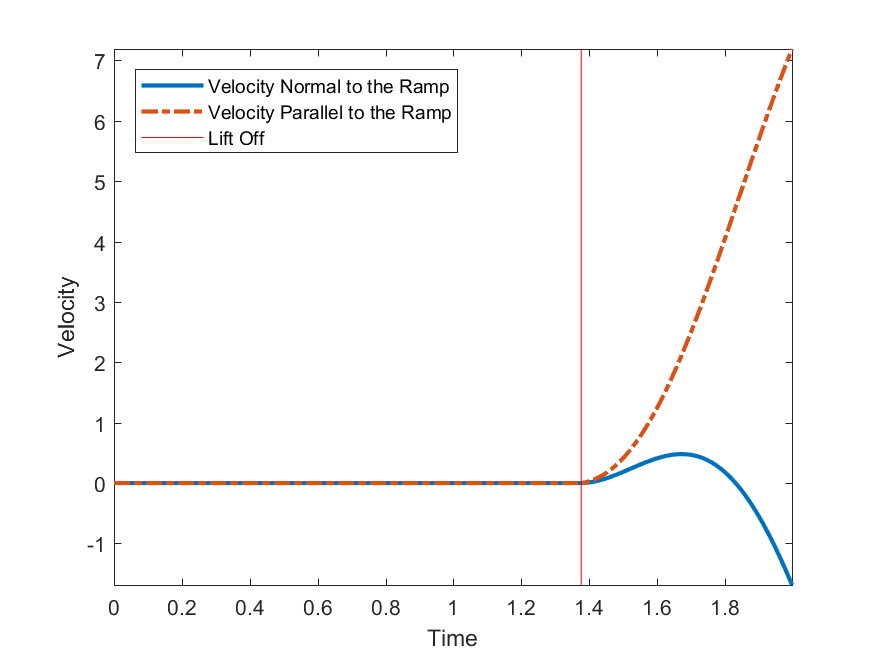
\includegraphics[height=3in]{img/constraint_check.png}
\caption{Plot of velocity relative to the slope showing no constraint violations prior to take off} 
\label{fig:constraint_check}
\end{figure}

\section{Coefficient of Friction}
\begin{figure}[h]
\centering
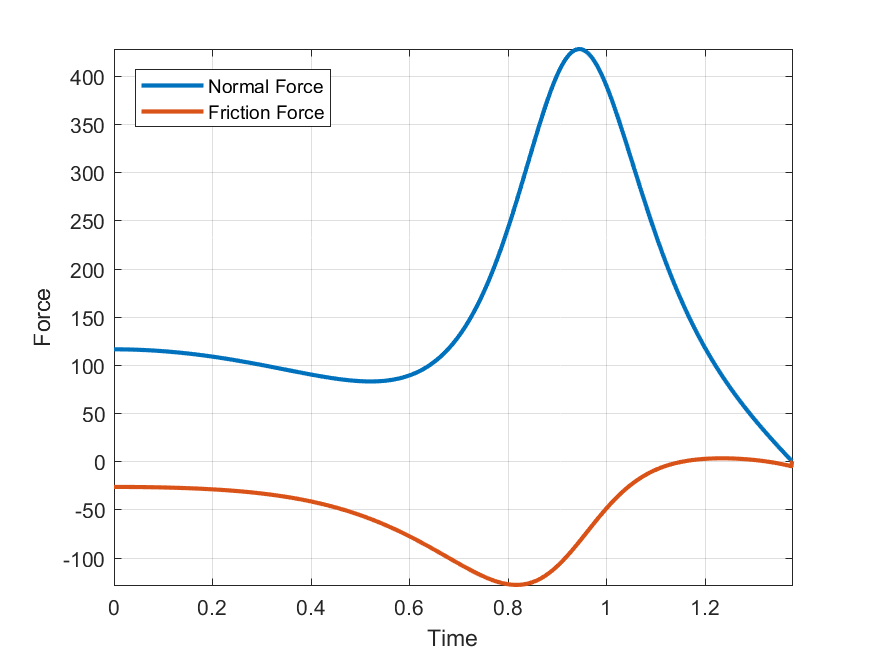
\includegraphics[height=3in]{img/constaint_force.png}
\caption{Constraint Force required for no slip motion}
\label{fig:constraint_force}	
\end{figure}

By taking the state information returned by ode45, and the DAE EOM (Eq \ref{eq:eom_dae}),  the constraint force can be computed for each time-step as shown in figure \ref{fig:constraint_force}.
Once the normal $F_n$ and friction $F_t$ force is known, the coefficient of friction can be computed using Eq. \ref{eq:friction_mu}.
As shown in figure \ref{fig:friction_mu}, $\mu \geq 0.895$ in order for the cylinder to roll with out slipping down the ramp.
\begin{equation}\label{eq:friction_mu}
\mu \geq \frac{F_t}{F_n}
\end{equation}

\begin{figure}[h]
\centering
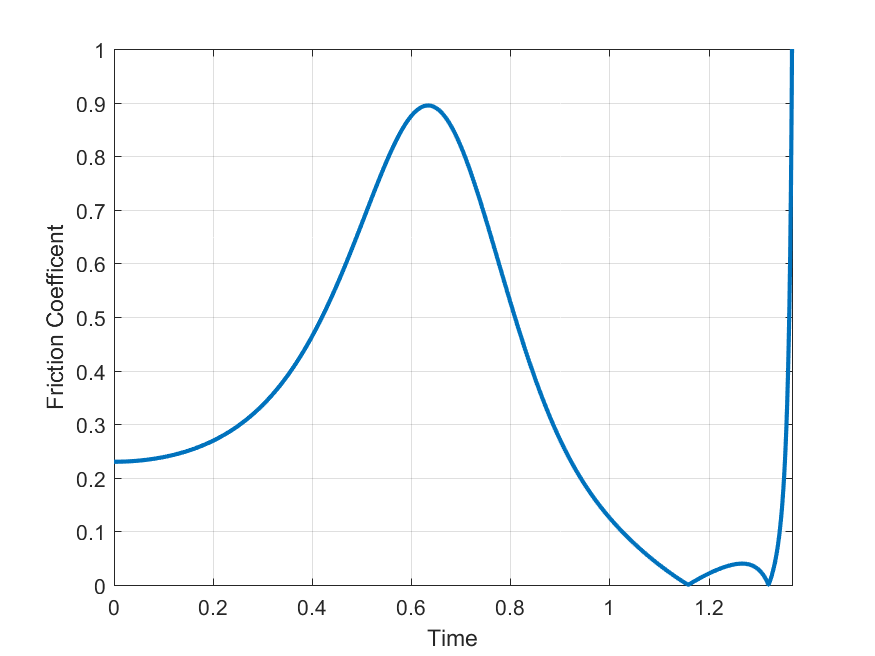
\includegraphics[height=3in]{img/friction_mu.png}
\caption{Required Friction Coefficient ($\mu$) at each time-step}
\label{fig:friction_mu}
\end{figure}

It should be noted that, as the cylinder approaches take off (The right side of Figure \ref{fig:friction_mu}), $F_n$ goes to zero and thus drives $\mu \to \infty$.
However, if we adopted the strict definition of equation \ref{eq:friction_mu}, then $mu$ would always be required to be infinite unless the cylinder did not jump.
Further, it seems reasonable to exclude the area where the friction model becomes discontinuous, in order to obtain a bounded value for $\mu$.

\section{Time to Take Off}
For the parameters used the cylinder rolled until $t = 1.3767$, before taking off.
This was determined by using events to integrate until the normal constraint force became negative.
As the ramp can only exert a positive normal force on the cylinder, a negative constraint force indicates that the cylinder was accelerating away from the map.
That is the cylinder has taken off and is no longer rolling down the ramp, and is instead flying through the air.

\section{Code}
All of the code used for this report can be found online at \url{github.com/awadell1/RollingEccentricCylinder}.
\begin{figure}[h]
\centering
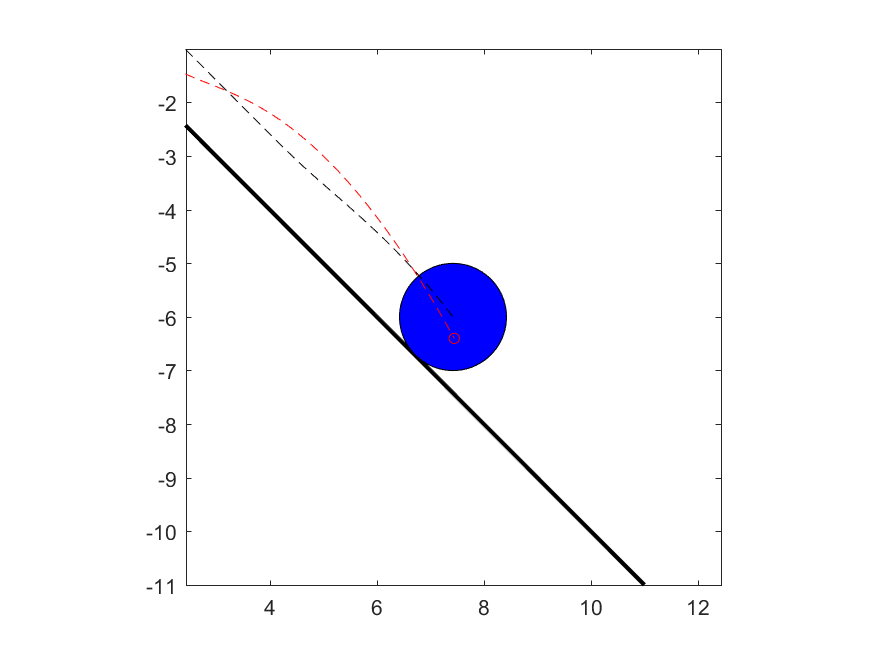
\includegraphics[height=3in]{img/animate.png}
\caption{Cylinder touching down after briefly flying through the air}
\label{fig:animate}
\end{figure}

%\subsection{Derive DAE}
%\MATLAB{deriveDAE.m}
%
%\subsection{Analysis}
%\MATLAB{analysis.m}
%
%\subsection{Simulate}
%\MATLAB{simulate.m}
%
%\subsection{RHS}
%\MATLAB{RHS_rolling.m}
%
%\subsection{DAE Matrices}
%\MATLAB{eom_rolling.m}
%
%\subsection{Energy Conservation}
%\MATLAB{energy_con.m}
%
%\subsection{Check Constraints}
%\MATLAB{constraint_violations.m}

\end{document}